\subsection{Saving Memory}
The aforementioned matrix \(A_d\) increases in size quickly for large \(n\) especially for \(d=3\), however, its entries are mostly zero. The SciPy library offers a matrix class which condenses a matrix by taking the nonzero entries and its indices. These matrix are called \textit{sparse}. We want to compare the memory usage for a dense and sparse matrix. This, of course, depends on the data type of the entries, the exact way how the class allocates memory et cetera, but we can at least formulate a way to count the nonzero entries for sparse matrices.

\begin{formula}
    Let \(d \in \{1, 2, 3\}\) be the number of the space dimension and \(n \in \mathbb{N}\) the number of grid points on each axis \([0, 1]\) excluding the start point, but including the end point (i.e. since the given problem has the value \(0\) at the boundary, we will effectively evaluate \((n - 1)^d\) points). Then, we have the formula for all entries of dense and the nonzero entries for sparse matrices
    \begin{align*}
        f^{(d = 1)}_{\text{dense}} (n) = (n - 1)^2 \hspace{0.5cm}&
        f^{(d = 1)}_{\text{sparse}} (n) = 3n - 5 \\
        %
        f^{(d = 2)}_{\text{dense}} (n) = (n - 1)^4 \hspace{0.5cm}&
        f^{(d = 2)}_{\text{sparse}} (n) = 5 (n - 1)^2 - 4 (n - 1) \\
        %
        f^{(d = 3)}_{\text{dense}} (n) = (n - 1)^6 \hspace{0.5cm}&
        f^{(d = 3)}_{\text{sparse}} (n) = 7 (n - 1)^3 - 6 (n - 1)^2 \text{.}
    \end{align*}

    \textit{Derivation} \hspace{0.1cm} The memory usage for dense matrix are precisely the number of elements of the matrix. Hence,
    \begin{align*}
        f^{(d)}_{\text{dense}} (n) =
        (n - 1)^d \cdot (n - 1)^d = (n - 1)^{2d}
    \end{align*}
    is the memory usage of the dense matrix.

    For sparse matrices, we consider each dimension separately. If \(d = 1\), then the diagonal containing \(2\) has \(n - 1\) elements. Additionally, the upper and lower diagonal shifted by one containing \(-1\) has each \(n - 2\) elements. Thus, we have
    \begin{align*}
        f^{(d = 1)}_{\text{sparse}} (n) & = (n - 1) + 2 (n - 2) \\
        & = 3n - 5 \text{.} 
    \end{align*}

    On the other hand, if \(d = 2\), then the matrix \(A_2\) contains \(n - 1\) times \(A_1\) with each having \(3n - 5\) elements. \(A_2\) also contains total of \(2 (n - 2)\) diagonal matrices with \(-1\) as entries which each again has \(n - 1\) elements. Summing all together, we have
    \begin{align*}
        f^{(d = 2)}_{\text{sparse}} (n) & = (n - 1) (3n - 5) + 2 (n - 2) (n - 1) \\
        & = 5 (n - 1)^2 - 4 (n - 1) \text{.}
    \end{align*}

    Lastly, if \(d = 3\), then the matrix \(A_3\) again contains \(n - 1\) times \(A2\) and \(2 (n - 2)\) diagonal matrices of the size \((n - 1)^2\). This gives us
    \begin{align*}
        f^{(d = 3)}_{\text{sparse}} (n) & = (n - 1) (5 (n - 1)^2 - 4 (n - 1)) + (2 (n - 2)) (n - 1)^2 \\
        & = 7 (n - 1)^3 - 6 (n - 1)^2 \text{.}
    \end{align*}
    \begin{flushright}
        \(\bigtriangleup\)
    \end{flushright}
\end{formula}
\begin{figure}[h]
    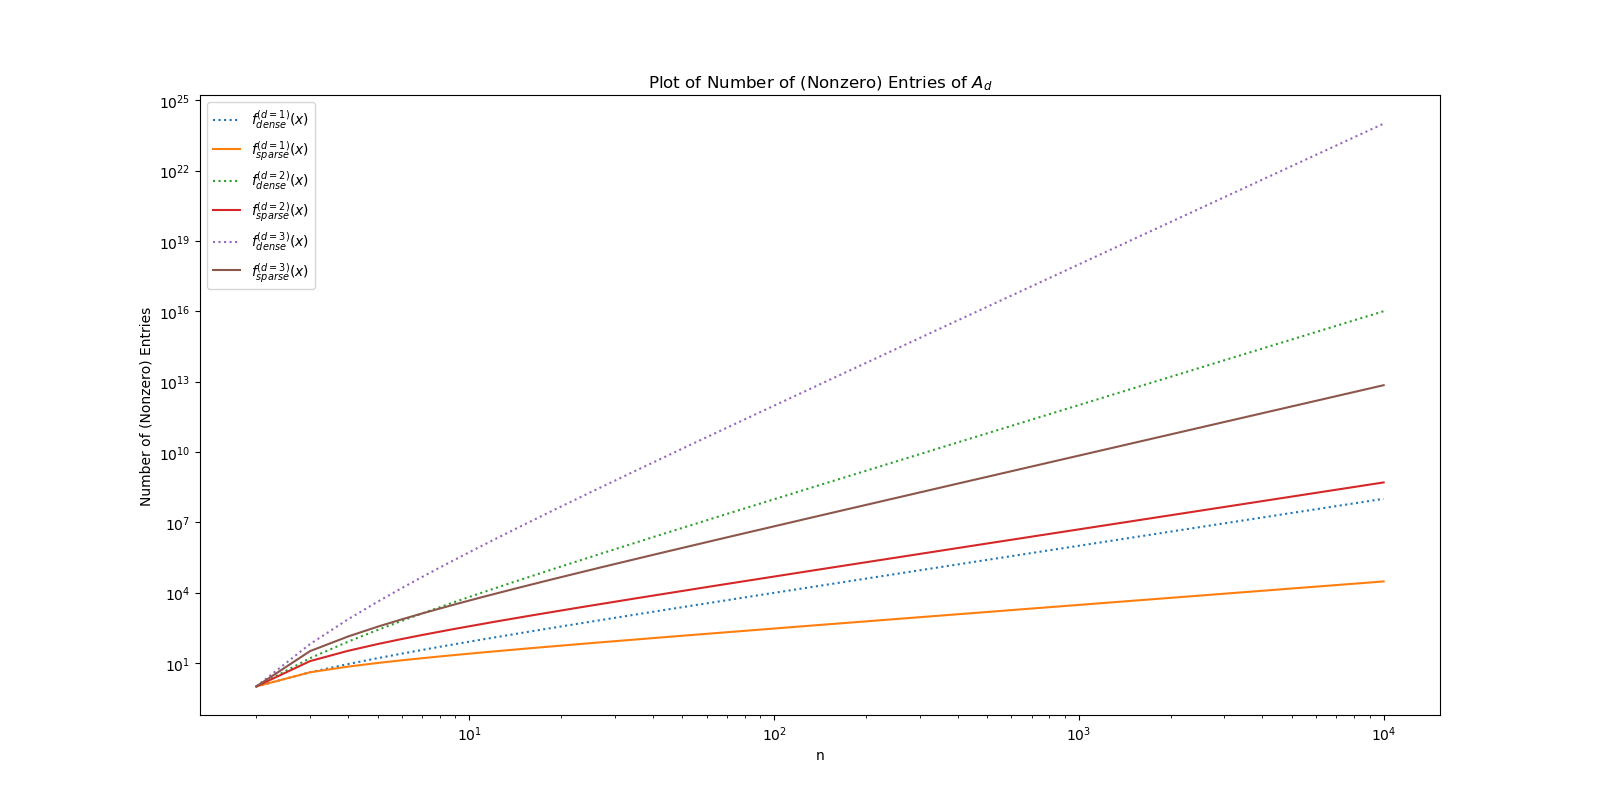
\includegraphics[width=\linewidth]{graphic/memory.png}
    \caption{The formula for the number of entries visualized.}
    \label{fig:plot}
\end{figure}
Perhaps the above formula might not be too exciting for some. For those, we have written a Python module \texttt{count\_entries.py} which visualizes the above formula for \(2 \leq n \leq 10000\) (see figure \ref{fig:plot}). One may change the \texttt{MAX\_N} variable to draw the graph for a different upper bound of \(n\).
